\section{Pierwszy program}

\begin{frame}[fragile]
  \frametitle{Pierwszy program}
  \framesubtitle{Witaj świecie!}

  Założenia pierwszego programu:

  \begin{itemize}
    \item uruchomienie wewnątrz przeglądarki internetowej
    \item osadzenie bezpośrednio w kodzie \textbf{HTML}
  \end{itemize}

\end{frame}


\begin{frame}[fragile]
  \frametitle{Pierwszy program}
  \framesubtitle{Witaj świecie!}

  Witaj świecie w \textbf{JavaScript}:

  \begin{minted}{html}
<html>
  <body>
    <script>
      alert('Witaj świecie!');
    </script>
  </body>
</html>
  \end{minted}

\end{frame}


\begin{frame}[fragile]
  \frametitle{Pierwszy program}
  \framesubtitle{Witaj świecie!}

  \begin{minted}[fontsize=\footnotesize]{html}
<html>
  <body>
    <script>
      alert('Witaj świecie!');
    </script>
  </body>
</html>
  \end{minted}

  \begin{itemize}
    \item 1--2, 6--7 --- HTML który już znamy
    \item \verb|<script>| -- znacznik zawierający skrypt
    \item 4 -- kod \textbf{JavaScript}
  \end{itemize}

\end{frame}


\begin{frame}[fragile]
  \frametitle{Pierwszy program}
  \framesubtitle{Witaj świecie!}

  \verb|alert(message)| --- powoduje wyświetlenie okna dialogowego w przeglądarce

  \begin{itemize}
    \item \verb|message| --- tekst który będzie wyświetlony w oknie (opcjonalny)
  \end{itemize}

  \begin{minted}{js}
alert('Ala ma kota');
  \end{minted}


  \begin{figure}
    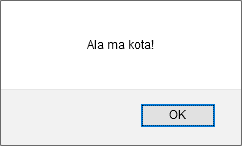
\includegraphics[scale=0.5]{images/js-alert-example}
  \end{figure}

\end{frame}

